\documentclass{article}
\usepackage[utf8]{inputenc}
\usepackage[T1]{fontenc}
\usepackage{color}
\usepackage{geometry}
\geometry{a4paper, left=1.8cm, right=2.0cm, top=1.1cm, bottom=2.2cm}
\usepackage{amssymb}
\usepackage{amsmath}
\usepackage{graphicx}
\usepackage[english]{babel}

\title{Group project - Linear model}
\author{Daniel Gilgen, David Lehnen, Matthias Roggo, Fabio Marti}
\date{\today}

\begin{document}
\maketitle
\parindent 0pt
\linespread{1.2} \selectfont
\numberwithin{equation}{section}
\parskip 10pt

We are considering a linear, timeinvariant model, given by the following circuit diagram

\begin{center}
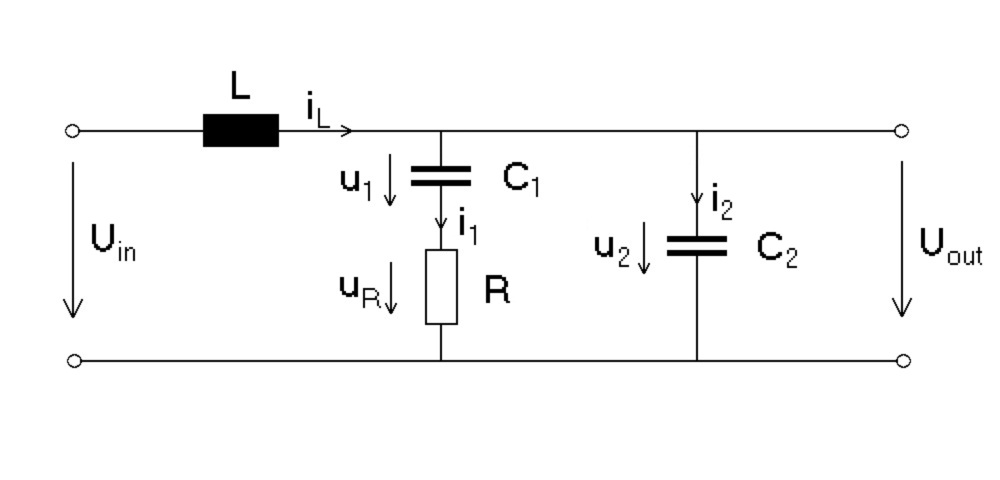
\includegraphics[width=14cm]{circuit_diagram}
\end{center}


This is obviously a system of order 3 with the states \(x_1 = i_L\), \(x_2 = u_1\) and \(x_3 = u_2\), the input \(u = U_{\text{in}}\) and the output \(y = U_{\text{out}}\). The system's equations are given by

\[L \cdot \frac{d i_L}{dt} = u_L = U_{\text{in}}-u_2\]

\[\Longrightarrow \qquad \frac{d i_L}{dt} = \frac{U_{\text{in}}}{L} - \frac{u_2}{L}\]

\[C_1 \cdot \frac{d u_1}{dt} = i_1 = u_R \cdot R = (u_2 - u_1) \cdot R\]

\[\Longrightarrow \qquad \frac{d u_1}{dt} = \frac{R}{C_1} \cdot u_2 - \frac{R}{C_1} \cdot u_1\]

\[C_2 \cdot \frac{d u_2}{dt} = i_2 = i_L - i_1 = i_L - (u_2 - u_1) \cdot R\]

\[\Longrightarrow \qquad \frac{d u_2}{dt} = \frac{i_L}{C_2} - \frac{R}{C_2} \cdot u_2 + \frac{R}{C_2} \cdot u_1\]

This leads to the following state space representation

\[ \left[
\begin{array}{c}
\dot{x}_1 \\
\dot{x}_2 \\
\dot{x}_3 \\
\end{array} \right]
= \left[
\begin{array}{c c c}
0 & 0 & -\frac{1}{L} \\
0 & -\frac{R}{C_1} & \frac{R}{C_1} \\
\frac{1}{C_2} & \frac{R}{C_2} & -\frac{R}{C_2} \\
\end{array}
\right]
\cdot \left[
\begin{array}{c}
x_1 \\
x_2 \\
x_3 \\
\end{array} \right]
+ \left[
\begin{array}{c}
\frac{1}{L} \\
0 \\
0 \\
\end{array} \right]
\cdot u
\]

\[
y = \left[
\begin{array}{c c c}
0 & 0 & 1 \\
\end{array}
\right] \cdot \left[
\begin{array}{c}
x_1 \\
x_2 \\
x_3 \\
\end{array} \right]
\]

What we have now is a continuous time state space model of the form

\[\dot{x}(t) = \bar{A}x(t) + \bar{B}u(t)\]
\[y(t) = \bar{C}x(t)\]

Now we can assume, that all electrical devices are not ideal or that there are external disturbances like fluctuations in temperature or air moisture, such that their behaviour is not ideal. These factors will lead to process noise \(w(t)\). Furthermore we will measure the output voltage \(U_{\text{out}}\) with a voltmeter, which will not measure the values exactly or which has an inappropriate resolution. This will add some measurement noise \(v(t)\) to our model. Our new state space representation will be

\[\dot{x}(t) = \bar{A}x(t) + \bar{B}u(t) + w(t)\]
\[y(t) = \bar{C}x(t) + v(t)\]

with

\[E[w(t)w(\tau)] = Q_e \delta(t-\tau)\]
\[E[v(t)v(\tau)] = R_e \delta(t-\tau)\]

so \(w(t)\) and \(v(t)\) are white Gaussian noise processes. Since we assume that our model is quite reliable and there are only few external disturbances, the process noise will be much smaller that the measurement noise. Reasonable choices for \(Q_e\) and \(R_e\) could be

\[
Q_e = \left[
\begin{array}{c c c}
10^{-4} & 0 & 0 \\
0 & 10^{-4} & 0 \\
0 & 0 & 10^{-4} \\
\end{array}
\right]
, \qquad\qquad R_e = 10^{-1}
\]

The last step is to convert this system into a discrete time linear system. The state space representation for such a system is given by

\[x_{k+1} = Ax_k + Bu_k + w_k\]
\[y_k = Cx_k + v_k\]

The matrices \(Q_e\) and \(R_e\) will stay the same. All other matrices are given by

\[A = e^{\bar{A} T}, \qquad\qquad\qquad B = \int_0^T e^{\bar{A} (T-\tau)} \bar{B} \;d\tau, \qquad\qquad\qquad C = \bar{C}\]

where \(T\) represents the sampling rate of our discrete time model. By choosing appropriate values for \(L\), \(C_1\), \(C_2\) and \(R\), we finally have enough information to build a Kalman filter for this linear system.



\end{document}